% Implementasjon

\chapter{Implementasjon} % Chapter title

\label{ch:implementasjon} % For referencing the chapter elsewhere, use \autoref{ch:mathtest}

% Formålet med dette kapittelet er å presentere vår implementasjon av løsningene av kravene vi skulle oppnå.
% Dette kapittelet vil også inneholde begrunnelser for valg.
%----------------------------------------------------------------------------------------


\section{Robot}

En autonom handlevogn er først og fremst et lite kjøretøy med utstyr for å kunne bevege seg i et typisk butikkmiljø.
At handlevognen skal gjøres autonom forutsetter en eller annen grad av kunstig intelligens. Denne kombinasjonen gjør
at handlevognen kan karakteriseres som en robot. Den må besitte aktuatorer \graffito{En aktuator gjør om elektrisk strøm
eller spenning til bevegelse} i form av motorer som beveger hjul eller belter for å bevege roboten rundt, og sensorer i
form av kollisjons- og posisjonsutstyr for å kunne navigere i miljøet. Den trenger også en intern eller ekstern prosessor
som kalkulerer handlinger for aktuatorene basert på data fra sensorer eller modeller.

Miljøet kan karakteriseres som delvis observerbart, stokastisk, kontinuerlig og kjent. Disse er begreper knyttet til
kunstig intelligens \cite{ai_modern_approach}. At miljøet er delvis observerbart vil si at at sensorene som roboten er utstyrt med vil kunne
kartlegge nesten alle aspekter ved miljøet, eksempelvis hindringer som mennesker, hyller, og andre store gjenstander
i veien. Mindre hindringer som grus, gjørme, nedoverbakker og trapper vil være vanskeligere å kartlegge. Stokastisk
vil si at tilstanden til verdenen ikke er entydig bestemt av robotens handlinger, men samtidig med menneskene som
beveger seg rundt i den. Miljøet er kontinuerlig, det vil si at bevegelser til aktører i verdenen skjer i sammenheng
med ekte tid, og ikke i diskrete episoder. Til sist karakteriseres miljøet som kjent. Dette betyr for eksempel at
roboten kan gjøre antagelser om at gulvet er flatt, at det finnes et oversiktlig rutenett av reoler, og at tilfeldige
hindringer av gjenstander og mennesker er relativt forutsigbare eller enkle å ta sporadisk hensyn til.

For å kutte utviklingstid ble det tatt i bruk en ferdig robot i form av en Pioneer 3-DX fra MobileRobots\footnote{\url{http://www.mobilerobots.com/}}. Gruppen så flere fordeler ved å ta i bruk denne: Åpen og godt dokumentert
utviklingsplattform, enkle grensesnitt mot alle de nyttige sensorene og aktuatorene ombord, godt utvalg av sensorer som
alle passet behovene for oppgaven. Grunnen til at valget falt på akkurat denne roboten i tillegg til de øvrige, var
fordi instituttet hadde tilgang på den og var villig til å låne den bort.

For å styre roboten ble operativsystemet ROS\footnote{\url{http://www.ros.org/}}, Robot Operating System, benyttet.
Dette er et open source operativsystem i utstrakt bruk blant robothobbyister. Følgelig er flere av modulene i det
beskrevne styringssystemet allerede utviklet, og kunne brukes uten større modifikasjoner.

\section{Posisjonering}

\begin{figure}[!ht]
  \centering
  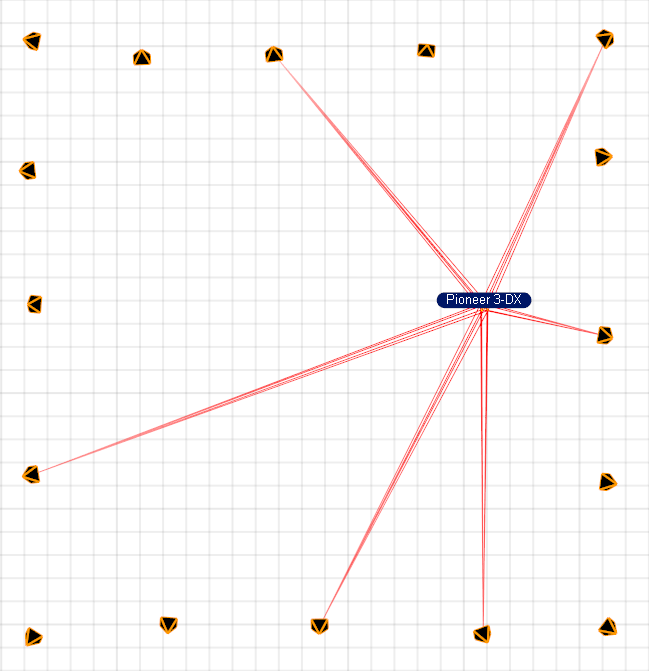
\includegraphics[width=0.75\textwidth]{gfx/mocap.png}
  \caption{Motion capture}
\end{figure}

For å posisjonere roboten i rommet ble det benyttet et motion capture system. Systemet var fast montert på rom
B333 og bestod av 16 infrarøde kamera av typen Flex 13 fra OptiTrack. Objekter som skulle spores ble utstyrt med markører som
reflekterte lys i det infrarøde området. Kameraene var utstyrt med infrarøde LED og hadde dermed mulighet til å posisjonere markørene i rommet. Ved å definere grupper av markører som stive
legemer kan systemet oppfatte både legemets posisjon og retning.

Et slikt system tilbød høy grad av presisjon, ned til få centimeter, men var også utsatt for støy i form av
lysforurensning. Området kameraene kunne spore et legeme var også
begrenset til noen få meter i hver retning fra midten av rommet.

Med kameraene fulgte det en programvarepakke som overførte posisjonen til de definerte legemene over nettverk
til datamaskinen som styrte roboten. Dataene ble importert i ROS og eksponert
som en topic. \graffito{Topics er ROS' implementasjon av meldingskanaler} Motion capture systemets
referanseramme samt posisjonen til roboten og posisjonen til brukeren ble overført på denne måten.

\section{Navigasjon}

\begin{figure}[!ht]
  \centering
  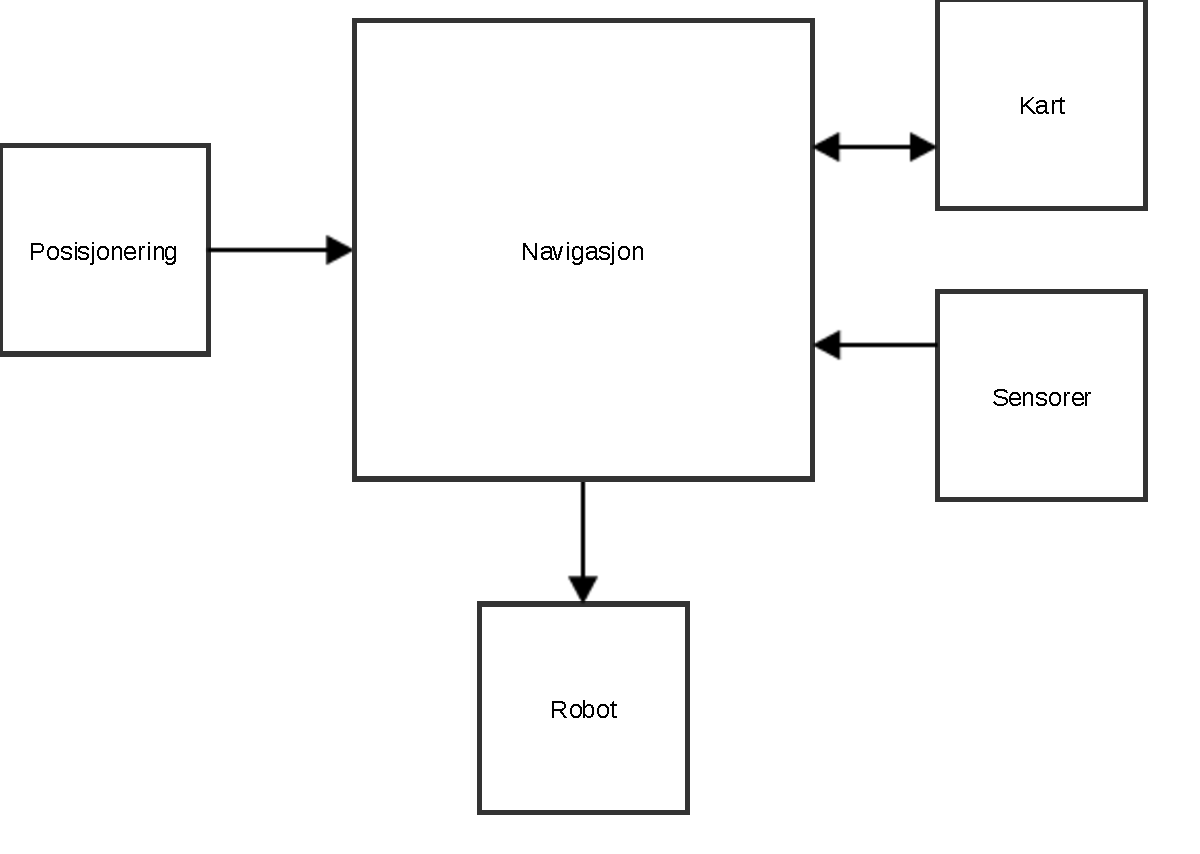
\includegraphics[width=\textwidth]{gfx/nav.pdf}
  \caption{Software stack}
  \label{fig:navstack}
\end{figure}

For å navigere roboten ble navigasjonspakken\footnote{\url{http://wiki.ros.org/navigation}} i ROS benyttet.
En oversikt over oppbygningen til denne pakken er vist i \autoref{fig:navstack}.
For å benytte dette systemet sammen med motion capture systemet ble systemets referanserammet overstyrt med den
fra motion capture anlegget, og inputkildene som kom inn fra venstre i \autoref{fig:navstack} var dermed ikke
relevante for den implementasjonen som ble benyttet.

Systemet mottok data fra lasermoduler og sonarmoduler for å orientere seg i forhold til hindringer i nærheten. 
Data fra sonar gav et lite detaljert bilde av omgivelsene, og var primært relevant for å detektere vegger
eller andre store hindringer. Laseren, vist i \autoref{fig:hokuyo}, hadde derimot oppløsning som gjorde at den kunne se også små hindringer. Knappene langs støtfangeren til roboten stanset bevegelse på et lavere nivå, slik at kjørekommandoer fra navigasjonssystemet ikke ble utført av roboten.

Ved bruk av sensordata fra laser og sonar bygde navigasjonssystemet et kostnadskart over omgivelsene, der hvert felt ble gitt
en verdi som indikerte kostnaden ved å forflytte seg gjennom feltet. Deretter benyttet systemet algoritmer for graftraversering
for å og benyttet dette da det planla en rute
frem til det gitte målet. Ruten ble planlagt i to stadier, globalt og lokalt. Den globale ruten ble generert
i det målet ble gitt til roboten, mens den lokale ruten ble oppdatert fortløpende etter som roboten tilegnet
seg ytterlige data om hindringer i omgivelsene. Om roboten møtte uforutsette hindringer forsøkte den å planlegge
en lokal rute rundt hindringen slik at den kom seg tilbake til den globale ruten. Om roboten etter en tid ikke
var i stand til å finne en slik rute vil den gi opp, og måtte gis et nytt mål før den kunne fortsette.

\begin{figure}[!ht]
  \centering
  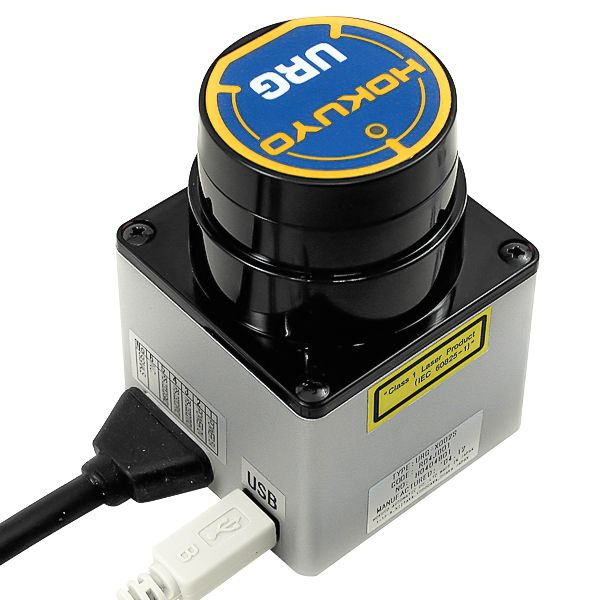
\includegraphics[width=0.5\textwidth]{gfx/hokuyo_urg_04lx.jpg}
  \caption[Hokuyo URG-04LX]{Hokuyo URG-04LX Scanning Laser Range Finder}
  \label{fig:hokuyo}
\end{figure}

For å gi roboten et mål å gå til ble to systemer utprøvd. Det første, for å teste funksjonalitet, bestod i å
gi roboten målpunkt ved å trykke på det ønskede målet i visualiseringsprogrammet RViz\footnote{\url{http://wiki.ros.org/rviz}}. Ved hjelp av dette var det på en enkel måte mulig å se hvordan
roboten tok seg frem til et mål, og hvordan den håndterte hindringer langs veien.
Et mer komplisert system som genererte målpunkter basert på bevegelsene til brukeren roboten skulle følge ble
også utprøvd, men aldri ferdigstilt i tilfredsstillende grad. Da
roboten bare kunne gis et mål av gangen bygde dette systemet en intern liste av målpunkter, og gav disse til
roboten ettersom roboten nådde det inneværende målpunktet. Dette ble implementert som en egen modul, knyttet sammen eksisterende moduler for å danne et komplett styringssystem til roboten.